\textbf{Creación de Máquina Virtual}
\begin{enumerate}

\item En primer lugar, elegimos el nombre de la máquina: \textbf{Cliente01} y el tipo, en este caso se trata de \textbf{Microsoft Windows} versión \textbf{Microsoft Windows 10 (64-bit)}.
\begin{figure}[H] %[H] para here [b] para bottom [t] para top
\begin{center}
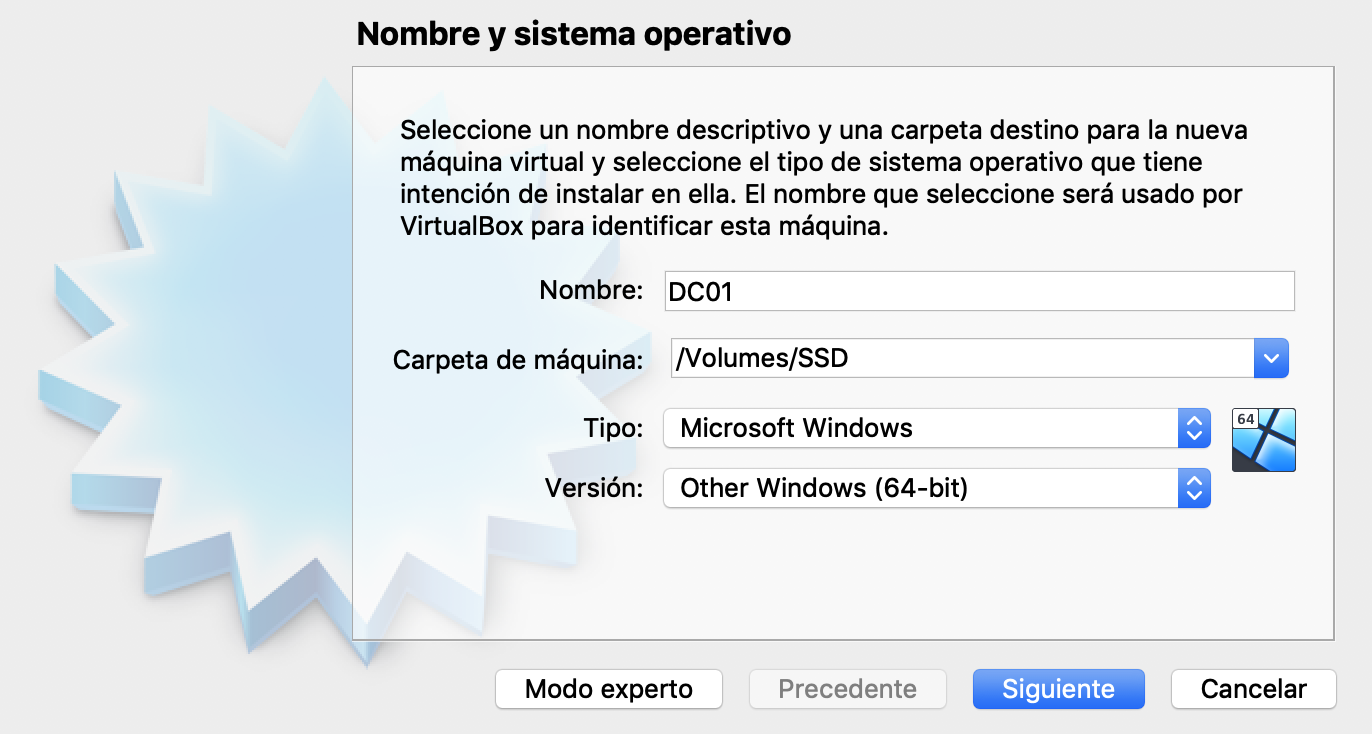
\includegraphics[width=10cm]{Cliente01/MV1.png}
\end{center}
\end{figure}

\item En el segundo paso, elegimos la RAM que vamos a destinar a la máquina virtual, aunque el requisito mínimo es de 2GB vamos a destinar 4GB: \textbf{4096 MB} para mejorar la experiencia a la hora de usar esta máquina.
\begin{figure}[H] %[H] para here [b] para bottom [t] para top
\begin{center}
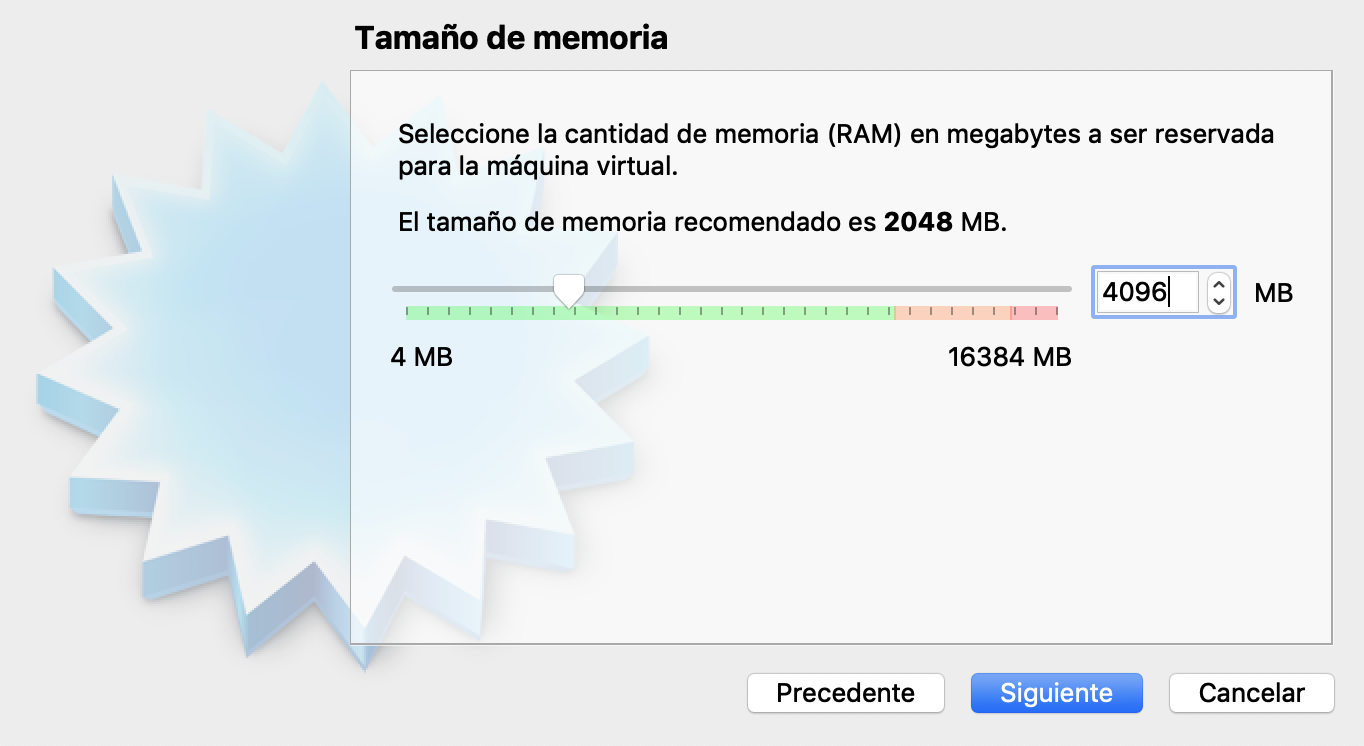
\includegraphics[width=10cm]{Cliente01/MV2.png}
\end{center}
\end{figure}

\item En esta opción, se elige \textbf{Crear un disco duro virtual ahora}.
\begin{figure}[H] %[H] para here [b] para bottom [t] para top
\begin{center}
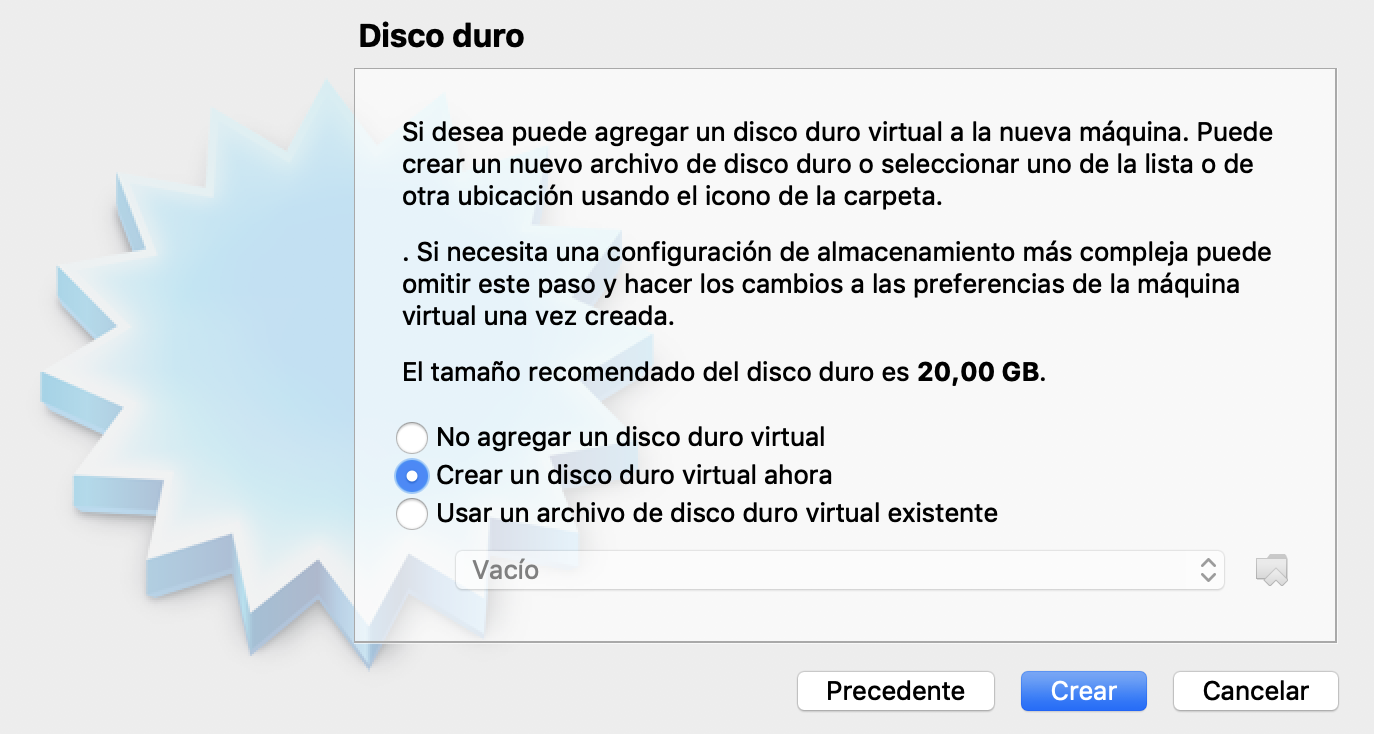
\includegraphics[width=10cm]{Cliente01/MV3.png}
\end{center}
\end{figure}

\item En cuanto al tipo de disco duro virtual se elige \textbf{VDI (Virtualbox Disk Image)}.
\begin{figure}[H] %[H] para here [b] para bottom [t] para top
\begin{center}
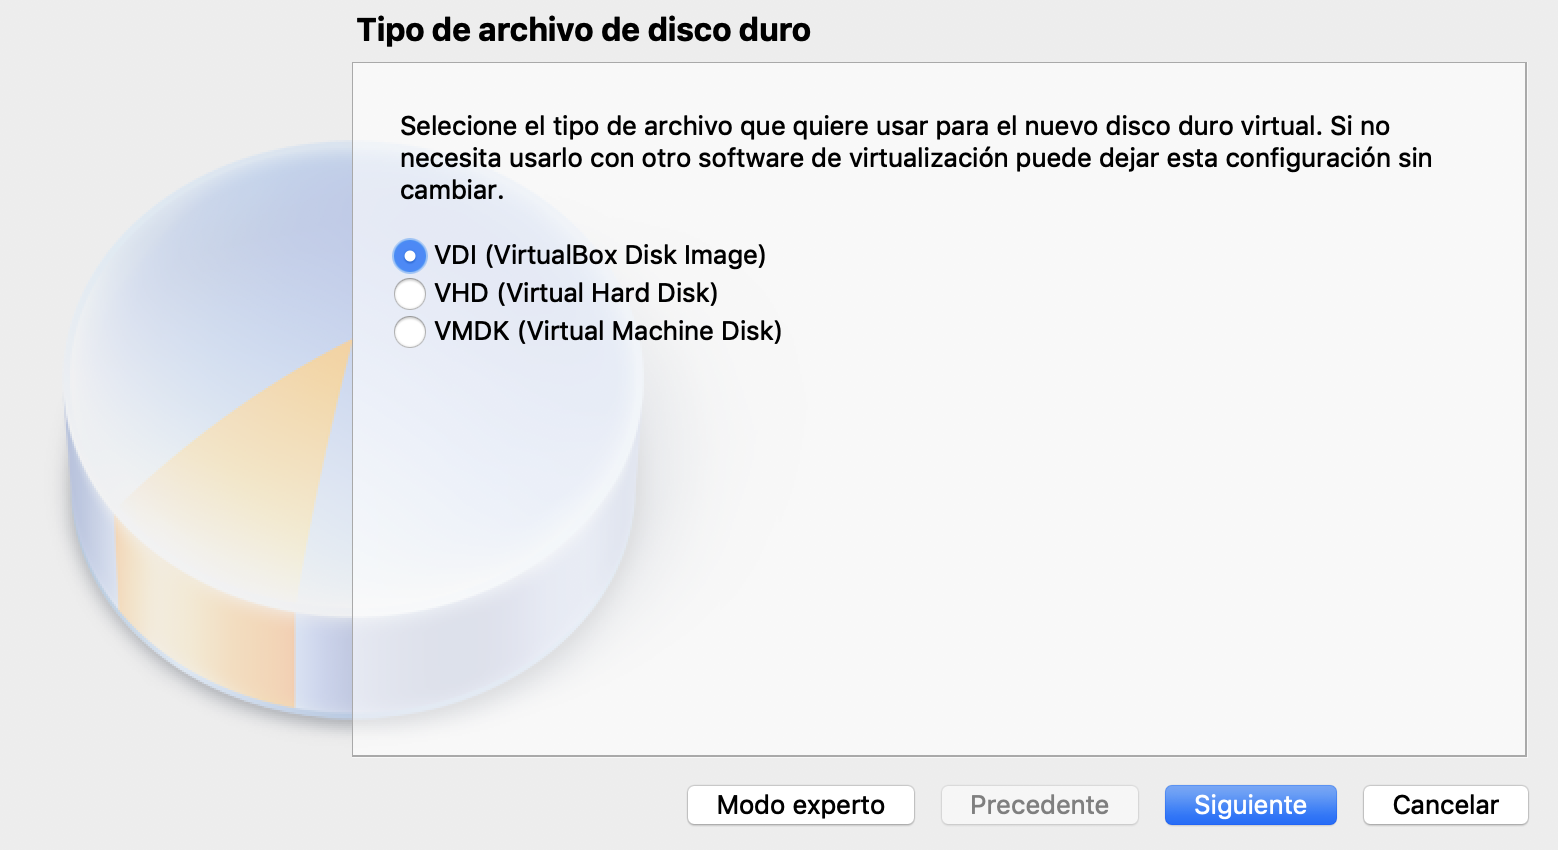
\includegraphics[width=10cm]{Cliente01/MV4.png}
\end{center}
\end{figure}

\item Por último, se ha elegido \textbf{30 GBs} de espacio de disco duro virtual.
\begin{figure}[H] %[H] para here [b] para bottom [t] para top
\begin{center}
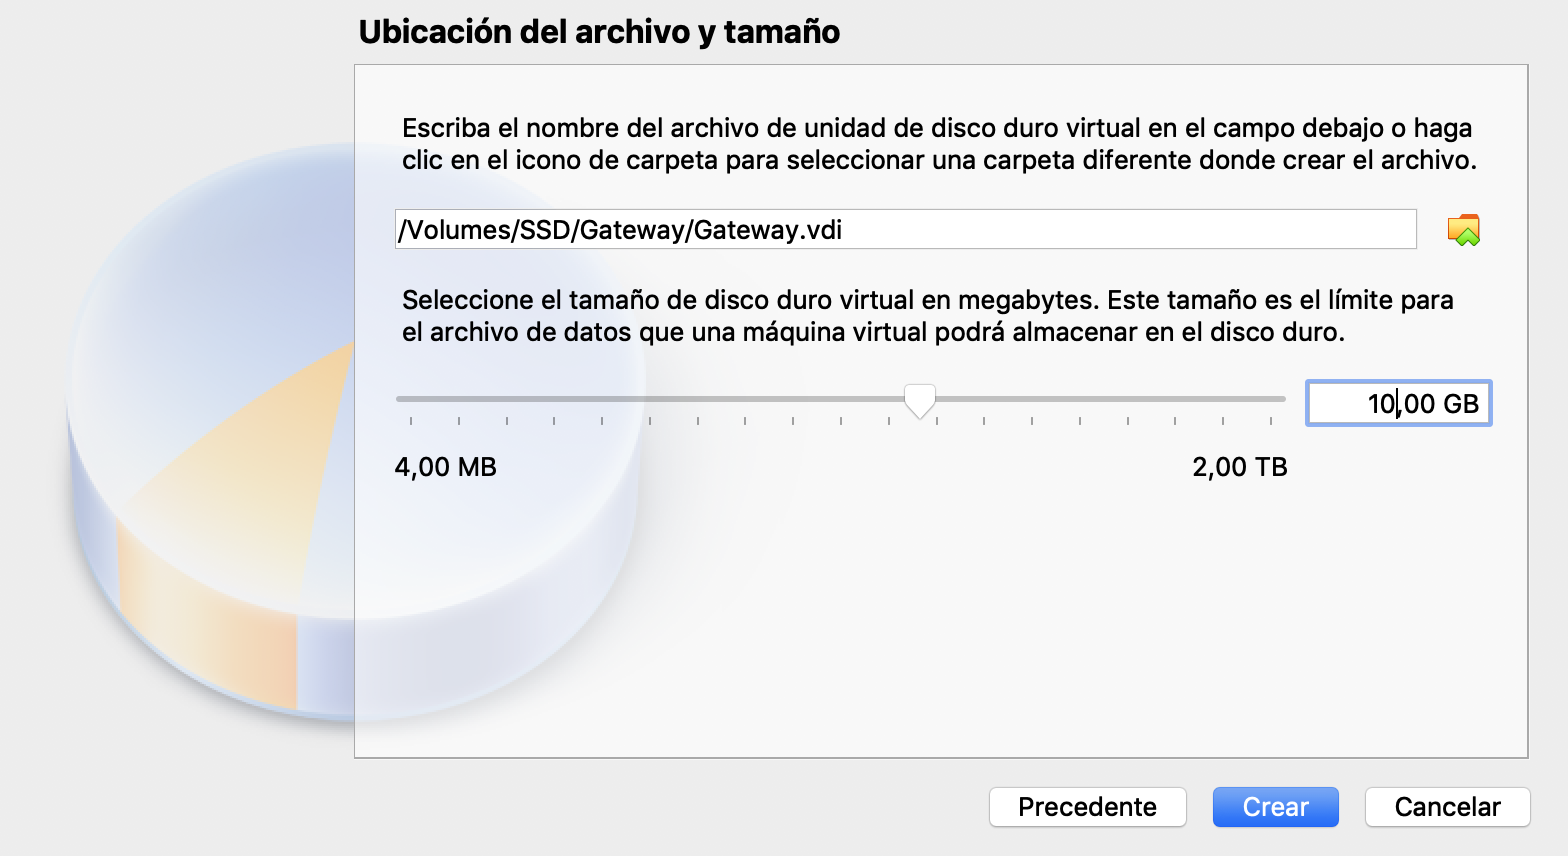
\includegraphics[width=10cm]{Cliente01/MV5.png}
\end{center}
\end{figure}

\item Para arrancar la imagen del sistema operativo, hay que seleccionarla desde Con\-fi\-gu\-ra\-ción/\-Almacenamiento de la máquina virtual creada como Unidad Óptica.
\begin{figure}[H] %[H] para here [b] para bottom [t] para top
\begin{center}
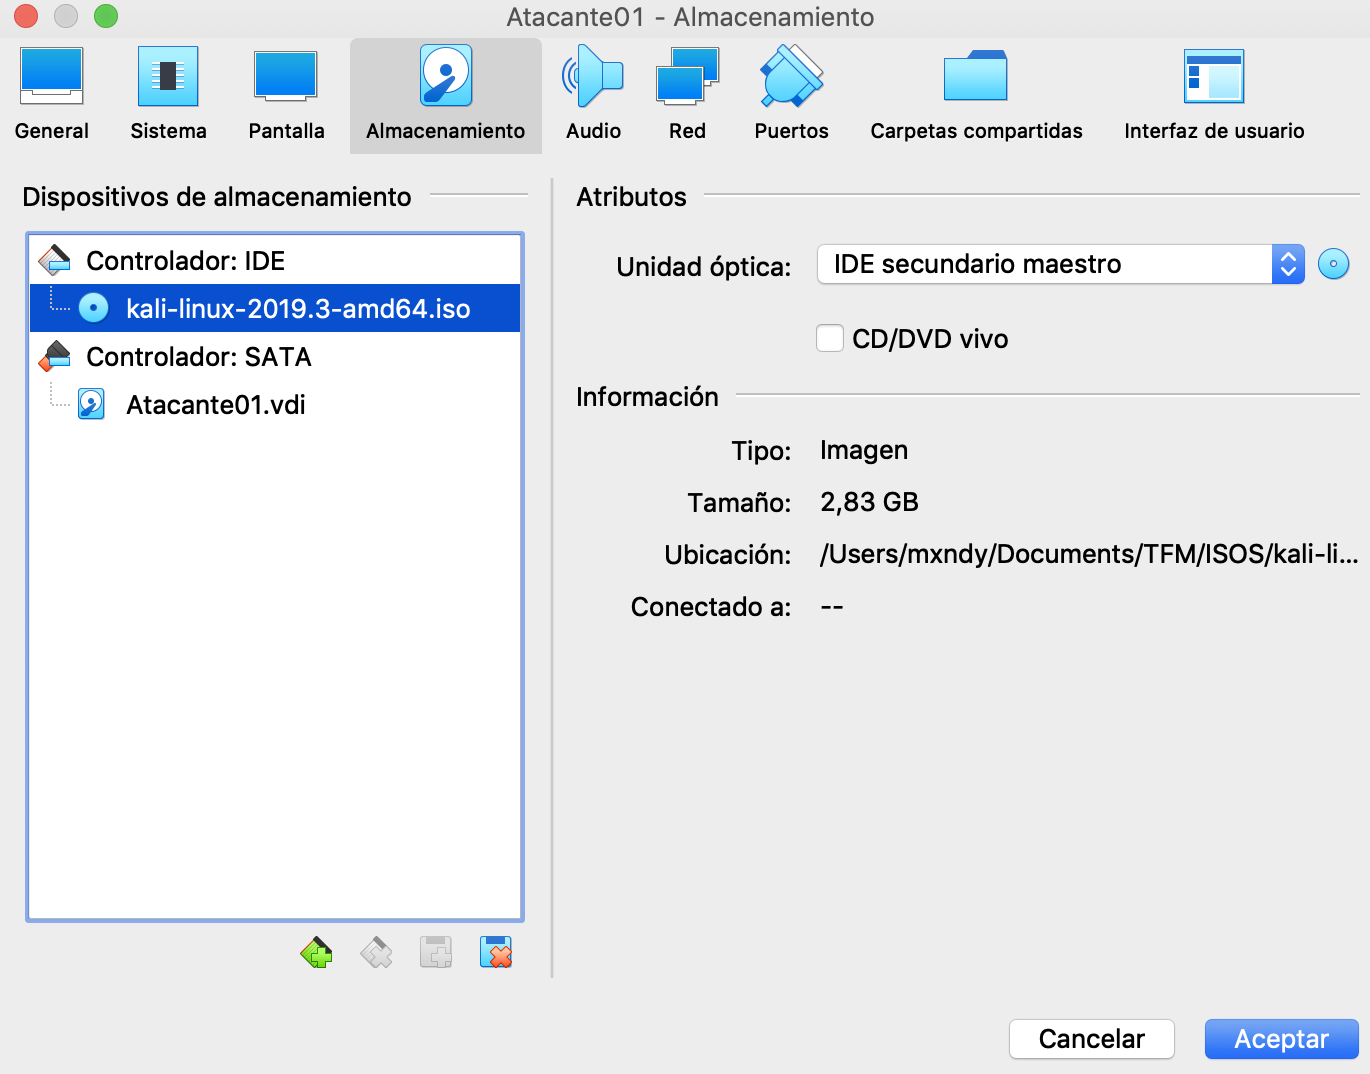
\includegraphics[width=10cm]{Cliente01/MV6.png}
\end{center}
\end{figure}




\end{enumerate}
\textbf{Instalación}

\textbf{Actualización}
